\cleardoublepage
\chapter{STUDI LITERATUR}
\label{chap:studi-literatur}

\section{Pemetaan Riset Terkait (\textit{State-of-the-Art})}

Dalam pengembangan pemodelan komputasi berbasis \textit{machine learning} untuk pemantauan lingkungan, transisi dari model regresi tunggal menuju arsitektur hibrida merupakan pendekatan yang banyak dikaji saat ini. Penempatan penelitian ini dalam khazanah literatur menjadi penting untuk memetakan posisi dan batasan dari pendekatan yang digunakan dibandingkan dengan penelitian-penelitian sebelumnya.

\subsection{Matriks Perbandingan Literatur Terkini}

Untuk mengevaluasi posisi metodologi penelitian ini, dilakukan tinjauan terhadap penelitian terdahulu dalam rentang lima tahun terakhir (2020--2025). Pemilihan literatur didasarkan pada relevansi penggunaan algoritma ansambel, pendekatan hibrida, serta studi kasus estimasi kualitas udara pada wilayah perkotaan. Tinjauan ini bertujuan untuk mempelajari perkembangan model prediktif sekaligus mengidentifikasi batasan dari metodologi yang ada sebagai acuan pengembangan sistem.

Perkembangan pemodelan dalam literatur menunjukkan kecenderungan pergeseran dari penggunaan algoritma tunggal ke arah arsitektur yang digabung (\textit{hybrid}) guna menangani sifat pola polutan yang tidak beraturan (non-linier). Meskipun demikian, terdapat variasi yang cukup besar dalam hal pemilihan fitur masukan dan metode penyetelan parameter. Kondisi ini menunjukkan bahwa pemahaman mengenai bagaimana suatu arsitektur merespons dinamika waktu dan lokasi yang berbeda masih terus berkembang.

Lebih lanjut, tren publikasi menunjukkan adanya perbedaan fokus dalam pemanfaatan fitur turunan tambahan. Sebagian besar literatur memproses polutan sebagai variabel yang berdiri sendiri secara statistik, tanpa mengaitkannya dengan reaksi kimiawi atmosferik di lapangan. Hal ini membatasi kemampuan model dalam merespons fluktuasi polusi akibat perubahan cuaca. Oleh karena itu, diperlukan tinjauan komparatif untuk memetakan cakupan fitur dan celah (\textit{gap}) dari masing-masing penelitian terdahulu, sebagaimana disajikan pada Tabel \ref{tbl:matriks_sota}.

\begin{table}[htbp]
\centering
\captionsetup{justification=centering}
\setlength{\tabcolsep}{5pt} 
\caption{Matriks Perbandingan Riset Terkait (\textit{State-of-the-Art}) Prediksi Kualitas Udara}
\label{tbl:matriks_sota}

\begin{tabularx}{\textwidth}{|>{\raggedright\arraybackslash}p{3.2cm}|
                              >{\raggedright\arraybackslash}p{2.2cm}|
                              >{\raggedright\arraybackslash}X|
                              >{\raggedright\arraybackslash}X|}
\hline
\textbf{Penulis} & \textbf{Metode} & \textbf{Fitur Utama} & \textbf{Celah Riset (\textit{Gap})} \\
\hline
\textcite{yenkikar2025explainable} & Hybrid RF-ARIMA & Polutan dasar & Mengabaikan interaksi antar-polutan. \\
\hline
\textcite{naz2024two} & \textit{Feature Engineering} & Turunan temporal & Ketiadaan koreksi residu temporal. \\
\hline
\textcite{alarsy2025pm25} & \textit{Random Forest} & Polutan mentah & Mengabaikan tren linier jangka panjang. \\
\hline
\textcite{chen2025hybrid} & \textit{Deep Learning} & \textit{Spatio-temporal attention} & Beban komputasi harian tinggi (GPU). \\
\hline
\textcite{radjabaycolle2025improving} & LSTM-SHAP & Memori sekuensial & Operasional terlalu kompleks untuk peladen lokal. \\
\hline
\end{tabularx}
\end{table}

\subsection{Identifikasi Kesenjangan Riset (\textit{Research Gap Analysis})}

Berdasarkan analisis komparatif pada Tabel \ref{tbl:matriks_sota}, terlihat bahwa meskipun metrik akurasi yang dihasilkan oleh berbagai pemodelan terdahulu cukup bervariasi, mayoritas pendekatan saat ini menitikberatkan pada sisi arsitektur komputasinya (\textit{model-centric}). Kondisi ini menyebabkan variabel polutan sering kali diproses oleh model sebagai representasi numerik murni tanpa memperhitungkan aspek keterkaitan fisik dan kimiawinya di atmosfer.

Hal tersebut dapat menyebabkan tidak tertangkapnya pola indikator penyebab polusi sekunder yang memengaruhi fluktuasi kualitas udara di wilayah tropis. Dari evaluasi literatur di atas, teridentifikasi tiga celah riset fundamental yang menjadi dasar pelaksanaan penelitian ini:

\begin{enumerate}
    \item {Pengabaian Interaksi Kimiawi:} Mayoritas penelitian (seperti pada studi \autocite{alarsy2025pm25} dan \autocite{yenkikar2025explainable}) hanya memasukkan parameter polutan secara individual ke dalam model. Faktanya, perubahan konsentrasi PM\textsubscript{10} di udara terbuka juga dipengaruhi oleh efek interaksi antar\-gas akibat radiasi matahari (\textit{fotolisis}). Celah ini mendasari penerapan \textit{feature engineering} untuk memetakan hubungan antar variabel tersebut.
    \item {Keterbatasan Fleksibilitas Arsitektur Model:} Pendekatan yang masih terpisah antara model statistik (ARIMA) yang linear atau \textit{ma\-chi\-ne lear\-ning} yang non\-li\-ne\-ar namun kurang menangkap pola autokorelasi pada data sisaan (\textit{residual}). Penggunaan arsitektur hibrida sekuensial untuk mengevaluasi data berjangka waktu panjang (15 tahun) di wilayah Jakarta masih terbatas dibahas.
    \item {Kebutuhan Efisiensi dan Transparansi:} Penelitian yang mengejar nilai akurasi menggunakan arsitektur \textit{Deep Learning} (seperti pada studi \autocite{chen2025hybrid}) memerlukan sumber daya komputasi yang besar dan sifatnya tidak transparan (\textit{black-box}). Pendekatan tersebut kurang sesuai untuk diterapkan pada sistem instansi lokal yang membutuhkan efisiensi operasional harian serta kejelasan dasar pengambilan keputusan melalui metode XAI.
\end{enumerate}
\section{Domain Sains Atmosfer dan Paradigma Regulasi ISPU}

Pemahaman mengenai parameter kualitas udara tidak dapat dilepaskan dari konteks sains atmosfer dan regulasi pemerintah yang mengaturnya. Bagian ini membahas karakteristik partikulat udara, kondisi spesifik polusi di Jakarta, standar pelaporan Indeks Standar Pencemar Udara (ISPU), serta mekanisme pembentukan polutan sekunder. Pemantauan kualitas udara secara global umumnya dilakukan terhadap \textit{Particulate Matter} (PM), yaitu campuran partikel padat dan cair yang melayang di udara. Partikel ini diklasifikasikan secara mendasar berdasarkan ukuran diameternya untuk menentukan sifat retensi dan perilakunya di udara \autocite{carb2025inhalable}. Pengelompokan ini diperlukan karena perbedaan dimensi fisik polutan memengaruhi karakteristik dispersi dan tingkat penetrasinya ke dalam organ pernapasan manusia. Perbandingan dimensi, sumber emisi, dan implikasi klinis secara lebih rinci antara dua jenis partikulat utama disajikan pada Tabel \ref{tbl:pm10vspm25}.

\begin{table}[htbp]
\centering
\captionsetup{justification=centering}
\setlength{\tabcolsep}{6pt} 
\caption{Perbandingan Karakteristik Polutan PM\textsubscript{10} dan PM\textsubscript{2,5}}
\label{tbl:pm10vspm25}

\begin{tabularx}{\textwidth}{|>{\raggedright\arraybackslash}p{2.8cm}|
                              >{\raggedright\arraybackslash}X|
                              >{\raggedright\arraybackslash}X|}
\hline
\textbf{Aspek Analisis} & \textbf{PM\textsubscript{10}} & \textbf{PM\textsubscript{2,5}} \\
\hline
Ukuran Fisik & Diameter $<$ 10 $\mu$m & Diameter $<$ 2,5 $\mu$m \\
\hline
Sumber Dominan & Debu jalan, aktivitas konstruksi, abrasi ban, dan proses mekanis. & Emisi kendaraan, proses pembakaran, dan reaksi fotokimia industri. \\
\hline
Tingkat Penetrasi & Mengendap di saluran pernapasan atas (trakeobronkial). & Menembus saluran pernapasan dalam hingga kantung alveoli. \\
\hline
Risiko Kesehatan & Iritasi saluran napas, eksaserbasi asma, dan PPOK (\textit{COPD}). & Penyakit kardiovaskular, stroke, dan risiko kanker paru-paru. \\
\hline
\end{tabularx}
\end{table}

Berdasarkan karakteristik fisik yang disajikan pada Tabel \ref{tbl:pm10vspm25}, profil risiko kesehatan dari partikulat ini menjadi aspek yang ditelaah secara mendalam dalam berbagai studi epidemiologi. Partikulat PM\textsubscript{10} dapat masuk ke sistem pernapasan bagian atas karena karakteristik fisisnya yang banyak dihasilkan dari proses mekanis, seperti debu jalan raya dan aktivitas konstruksi harian \autocite{firdaus2023jakarta}. Penelitian oleh \textcite{zhang2021association} menunjukkan bahwa setiap kenaikan konsentrasi PM\textsubscript{10} sebesar 10 µg/m³ berkaitan dengan kecenderungan kenaikan jumlah kunjungan gawat darurat akibat penyakit kardiovaskular sebesar 0,14\%. Sementara itu, \textcite{kyung2020particulate} menemukan bahwa paparan terhadap PM\textsubscript{10} berkorelasi dengan adanya perubahan angka rawat inap pasien Penyakit Paru Obstruktif Kronis (PPOK) sebesar 2,7\%.

Kecenderungan data statistik dan rekam medis tersebut menunjukkan bahwa pemantauan dan penyediaan informasi proyeksi kualitas udara diperlukan untuk mendukung langkah preventif, khususnya bagi kelompok masyarakat yang rentan. Hal ini menjadi relevan bagi wilayah dengan tingkat aktivitas urban yang padat seperti DKI Jakarta, di mana akumulasi emisi harian berpotensi memengaruhi kondisi kesehatan publik dalam jangka panjang. Oleh karena itu, analisis pemodelan untuk mengestimasi konsentrasi polutan ini diposisikan sebagai pendekatan teoretis dan eksperimental guna menyediakan acuan data yang dapat ditelaah secara terukur bagi pengelolaan lingkungan perkotaan.

\subsection{Krisis Polusi Jakarta dan Integritas Dataset}
DKI Jakarta tercatat sebagai salah satu kota dengan tingkat polusi udara yang tinggi di kawasan Asia Tenggara. Berbeda dengan kota-kota di lintang subtropis, kondisi polusi di Jakarta dipengaruhi oleh iklim tropis dan pola angin muson. Menurut \textcite{firdaus2023jakarta}, konsentrasi polutan mengalami kenaikan selama musim kemarau. Pada periode tersebut, fenomena inversi suhu menahan gas buang dari kendaraan bermotor dan industri di lapisan udara bawah kota. Kondisi ini sejalan dengan data Kementerian Kesehatan RI yang mencatat bahwa kualitas udara Jakarta dapat masuk ke dalam zona "Tidak Sehat" \autocite{kemkes2019air, aulia2024air}.

Dalam perancangan model sains data berbasis deret waktu (\textit{time series}), validitas hasil estimasi bergantung pada kelengkapan data historis. Penelitian ini menggunakan data Indeks Standar Pencemar Udara (ISPU) Jakarta untuk periode 2010--2025 \autocite{pohan2025jakarta}. Pemilihan PM\textsubscript{10} sebagai target utama prediksi didasarkan pada tingkat keandalan instrumen pemantauan di lapangan. Data polutan PM\textsubscript{2,5} di Jakarta sebelum tahun 2020 memiliki tingkat data kosong (\textit{missing values}) yang mencapai 73\%. Kondisi ini kurang ideal untuk melatih algoritma deret waktu yang membutuhkan kesinambungan data kronologis. Sebaliknya, parameter PM\textsubscript{10} memiliki tingkat keterisian data yang tinggi, yaitu 94\% observasi valid sejak tahun 2010, sehingga menjadi variabel yang stabil untuk digunakan dalam pemodelan.

\subsection{Kalkulasi Indeks Standar Pencemar Udara (ISPU)}

Untuk mempermudah penyampaian informasi tingkat polusi kepada masyarakat, Kementerian Lingkungan Hidup dan Kehutanan (KLHK) menggunakan indikator Indeks Standar Pencemar Udara (ISPU) \autocite{chaniago2020ispu}. Berdasarkan Peraturan Menteri LHK No. P.14 Tahun 2020 \autocite{permenlhk2020ispu}, ISPU didefinisikan sebagai angka tanpa satuan (dari 0 hingga lebih dari 300) yang merangkum tingkat pencemaran dari berbagai indikator utama melalui mekanisme interpolasi linear bersegmen.

Penelitian Tugas Akhir ini difokuskan secara langsung pada prediksi nilai konsentrasi numerik mentah dari partikulat PM\textsubscript{10} ($\mu\text{g/m}^3$) dan bukan pada angka indeks transformasi ISPU. Pendekatan ini dipilih guna menjaga granularitas varians data asli agar tidak tereduksi oleh fungsi pembagian segmen regulasi, sehingga algoritma komputasi dapat mempelajari pola fluktuasi secara lebih sensitif. Namun, klasifikasi kategori mutu udara berdasarkan rentang nilai regulasi tetap dimanfaatkan sebagai acuan dasar dalam memetakan tingkat risiko lingkungan di DKI Jakarta, sebagaimana disajikan pada Tabel \ref{tbl:ispu}.

\begin{table}[htbp]
\centering
\captionsetup{justification=centering}
\setlength{\tabcolsep}{6pt} 
\caption{Kategorisasi ISPU dan Dampak Kesehatan Spesifik}
\label{tbl:ispu}

\begin{tabularx}{\textwidth}{|>{\raggedright\arraybackslash}p{2.3cm}|
                              >{\raggedright\arraybackslash}p{3.2cm}|
                              >{\raggedright\arraybackslash}X|}
\hline
\textbf{Rentang Indeks} & \textbf{Kategori Mutu} & \textbf{Dampak dan Implikasi Kesehatan} \\
\hline
0 -- 50 & Baik & Tidak memberikan efek negatif bagi kesehatan manusia, hewan, atau tumbuhan. \\
\hline
51 -- 100 & Sedang & Kualitas udara dapat diterima; berpotensi memengaruhi kelompok tumbuhan yang sensitif. \\
\hline
101 -- 200 & Tidak Sehat & Merugikan kesehatan umum, terutama kelompok rentan (bayi, lansia, dan penderita asma). \\
\hline
201 -- 300 & Sangat Tidak Sehat & Risiko tinggi penurunan fungsi paru serta memicu masalah kesehatan masyarakat yang lebih luas. \\
\hline
$>$ 300 & Berbahaya & Tingkat kritis; memicu keadaan darurat kesehatan serta gangguan pernapasan serius pada populasi. \\
\hline
\end{tabularx}
\end{table}

Keterbatasan utama dari mekanisme pelaporan ISPU saat ini adalah sifatnya yang reaktif \autocite{septiani2024combating}. Nilai ISPU yang dipublikasikan merupakan hasil perhitungan rata-rata dari kondisi kualitas udara selama 24 jam ke belakang. Artinya, mekanisme tersebut bersifat retrospektif karena mencerminkan akumulasi nilai masa lalu, sehingga belum menyediakan informasi prediktif untuk periode mendatang. Keterbatasan ini menjadi alasan mengapa integrasi pendekatan \textit{machine learning} digunakan untuk membantu membangun pemodelan estimasi dini yang proaktif.

\subsection{Mekanisme Fotokimia: Justifikasi Interaksi Fitur Komposit}

Dinamika partikulat di udara perkotaan tidak hanya ditentukan oleh emisi pembuangan langsung, tetapi juga oleh pembentukan partikel sekunder melalui reaksi kimia di udara. Di wilayah beriklim tropis seperti Jakarta, radiasi ultraungu (UV) dari matahari bertindak sebagai pemicu reaksi fotokimia. Reaksi ini mengubah gas polutan menjadi partikel padat PM\textsubscript{10}. Pemahaman mengenai reaksi kimia ini menjadi landasan untuk melakukan proses rekayasa fitur (\textit{feature engineering}) pada model prediksi yang dikembangkan.

Dalam rantai reaksi tersebut, gas Karbon Monoksida (CO) dan Ozon (O\textsubscript{3}) memiliki keterkaitan. CO digunakan sebagai indikator besarnya aktivitas emisi primer kendaraan sekaligus agen yang mempercepat reaksi kimia di udara. Di sisi lain, O\textsubscript{3} di permukaan tanah terbentuk dari hasil reaksi gas buang kendaraan akibat paparan radiasi matahari. Apabila konsentrasi gas CO dan O\textsubscript{3} berada pada tingkat yang tinggi dalam waktu yang bersamaan, kondisi ini mengindikasikan bahwa proses pembentukan polutan sekunder di udara sedang berlangsung, yang memengaruhi fluktuasi konsentrasi PM\textsubscript{10}.

Pembuatan fitur turunan baru yang merupakan hasil kali interaksi antara gas tersebut ($CO \times O_3$) bertujuan untuk mendeteksi kondisi atmosferik yang reaktif tersebut. Secara komputasi, fitur tambahan ini memberikan informasi varians tambahan kepada algoritma \textit{Random Forest} untuk mengenali pola pembentukan polusi sekunder. Penggunaan fitur interaksi kimiawi ini ditujukan untuk meminimalkan kesalahan prediksi pada saat terjadinya lonjakan polusi mendadak \autocite{naz2024two}. Dengan demikian, model memasukkan representasi karakteristik fisik dan kimia yang terjadi di atmosfer perkotaan.

\section{Fondasi Teoretis Analisis Deret Waktu (\textit{Time Series Analysis})}

Pemodelan kualitas udara pada dasarnya merupakan analisis data deret waktu (\textit{time series}). Deret waktu PM\textsubscript{10} ($Y_t$) didefinisikan sebagai sekumpulan variabel observasi yang diindeks berdasarkan urutan waktu ($t$). Prinsip utama dari analisis ini adalah asumsi bahwa nilai observasi pada waktu saat ini ($t$) memiliki keterikatan atau korelasi dengan nilai observasi pada rentang waktu sebelumnya ($t-k$) \autocite{vasconcelos2025stationarity}.

\subsection{Karakteristik Komponen Temporal}

Konsentrasi PM\textsubscript{10} di wilayah perkotaan merupakan perpaduan dari beberapa pola pergerakan temporal yang terjadi secara bersamaan. Secara teoretis, fluktuasi data runtun waktu dapat dipisahkan secara konseptual menjadi komponen tren jangka panjang (yang mencerminkan arah pergerakan pola emisi perkotaan secara perlahan) dan komponen musiman (yang berulang secara periodik mengikuti siklus iklim harian, mingguan, atau bulanan). Pemahaman terhadap karakteristik fluktuasi ini diperlukan agar pemodelan dapat memetakan dinamika data secara lebih terstruktur.

Pemisahan konseptual antara komponen pergerakan jangka panjang dan pola fluktuasi periodik ini menjadi landasan teoretis bagi penerapan arsitektur model hibrida sekuensial pada penelitian ini. Pemodelan tidak menggunakan fungsi dekomposisi statistik klasik secara formal, melainkan mengadopsi pendekatan asimilasi komponen varians. Algoritma \textit{machine learning} berbasis pohon keputusan digunakan pada tahap awal untuk memetakan pola fluktuasi non-linier jangka pendek yang dipengaruhi oleh rekayasa fitur temporal. Selanjutnya, model statistik ARIMA difokuskan untuk menangkap sisaan pola autokorelasi linier yang belum terpetakan oleh model pertama guna meminimalkan nilai galat estimasi.

\subsection{Prinsip Stasioneritas dan Formulasi Pengujian ADF}

Syarat dalam menggunakan model statistik linier seperti ARIMA adalah data deret waktu harus bersifat stasioner. Sebuah data deret waktu dikatakan stasioner apabila karakteristik statistiknya, seperti nilai rata-rata (\textit{mean}) dan ragam (\textit{variance}), konstan seiring berjalannya waktu \autocite{minitab2025adf}. Jika syarat stasioneritas ini tidak terpenuhi, model prediksi dapat menghasilkan estimasi yang kurang akurat.

Untuk memastikan apakah sebuah data sudah stasioner, pengujian dilakukan secara statistik menggunakan uji \textit{Augmented Dickey-Fuller} (ADF) \autocite{vasconcelos2025stationarity}. Uji ADF bekerja dengan mendeteksi ada tidaknya akar unit (\textit{unit root}) pada data. Evaluasi ini dilakukan menggunakan model regresi yang diturunkan pada Persamaan \ref{eq:adf}.

\begin{equation}
\Delta y_t = \alpha + \beta t + \gamma y_{t-1} + \sum_{i=1}^{p} \delta_i \Delta y_{t-i} + \epsilon_t
\label{eq:adf}
\end{equation}
\eqcaption{Formulasi Regresi Uji \textit{Augmented Dickey-Fuller} (ADF)}

\newpage

Hasil dari perhitungan uji ADF dievaluasi melalui nilai probabilitas (\textit{p-value}). Hipotesis nol ($H_0$) pada pengujian ini menyatakan bahwa data memiliki akar unit (tidak stasioner). Jika nilai \textit{p-value} yang dihasilkan lebih kecil dari 0,05, maka $H_0$ ditolak, yang mengonfirmasi bahwa data PM\textsubscript{10} telah stasioner sehingga pemodelan menggunakan ARIMA dapat dilakukan.

\subsection{\textit{Autocorrelation} dan \textit{Partial Autocorrelation Function} (ACF \& PACF)}

Identifikasi korelasi waktu digunakan untuk memahami hubungan antara kualitas udara di masa lalu terhadap kondisi saat ini. Dalam pemodelan statistik, parameter model ditentukan dengan menganalisis nilai autokorelasi pada data tersebut. 

\textit{Autocorrelation Function} (ACF) mengukur tingkat korelasi antara nilai observasi saat ini ($y_t$) dengan nilai observasi pada masa lalu ($y_{t-k}$) pada berbagai interval waktu jeda (\textit{lag}). Formulasi matematis untuk menghitung koefisien ACF diturunkan pada Persamaan \ref{eq:acf}.

\begin{equation}
\rho_k = \frac{\sum_{t=k+1}^T (y_t - \bar{y})(y_{t-k} - \bar{y})}{\sum_{t=1}^T (y_t - \bar{y})^2}
\label{eq:acf}
\end{equation}
\eqcaption{Formulasi Koefisien \textit{Autocorrelation Function} (ACF)}

Sementara itu, \textit{Partial Autocorrelation Function} (PACF) mengukur korelasi antara observasi saat ini ($y_t$) dengan observasi masa lalu ($y_{t-k}$), tanpa memperhitungkan pengaruh dari jeda waktu yang berada di antaranya. Analisis kombinasi dari grafik ACF dan PACF digunakan sebagai instrumen untuk membantu menentukan batasan orde model (\textit{p} dan \textit{q}) dalam algoritma ARIMA.

\section{Taksonomi Algoritma Regresi dan Teori Hibridisasi}

Pemodelan data deret waktu PM\textsubscript{10} berhadapan dengan dua karakteristik utama, yaitu pola non-linier yang dipicu oleh fluktuasi cuaca serta interaksi antar-polutan, dan pola linier dari tren jangka panjang. Oleh karena itu, pendekatan teoretis dalam penelitian ini menggabungkan algoritma \textit{machine learning} berbasis pohon keputusan dan model statistik klasik.

\subsection{Algoritma \textit{Random Forest Regressor}}

\textit{Random Forest} (RF) merupakan algoritma \textit{ensemble learning} yang bekerja dengan menggabungkan sekumpulan pohon keputusan (\textit{Decision Trees}) untuk menghasilkan prediksi akhir dengan nilai kesalahan yang rendah \autocite{alarsy2025pm25, abdallah2025predicting}. Algoritma ini dirancang untuk mereduksi masalah varians tinggi (\textit{overfitting}) yang dapat terjadi jika hanya menggunakan satu pohon keputusan tunggal. RF menjaga stabilitas estimasi melalui dua proses acak utama:

\begin{enumerate}
    \item {\textit{Bootstrap Aggregating} (Bagging):} Setiap pohon keputusan di dalam model dilatih menggunakan sebagian baris data sampel acak berukuran $N$ yang diambil dengan pengembalian (\textit{with replacement}). Sekitar 36,8\% data yang tidak terambil oleh sebuah pohon disebut sebagai data \textit{Out-of-Bag} (OOB), yang dimanfaatkan untuk proses validasi internal model.
    \item {\textit{Random Subspace Method}:} Pada setiap proses penentuan cabang (\textit{node splitting}), algoritma membatasi jumlah variabel fitur yang diuji. Jika terdapat $M$ total fitur, algoritma hanya memilih sebagian fitur (umumnya $\sqrt{M}$ atau $M/3$) secara acak. Proses ini meminimalkan dominasi dari satu fitur tertentu, sehingga pohon-pohon yang dihasilkan menjadi lebih bervariasi secara independen.
\end{enumerate}

\bigskip

Dalam setiap pembentukan pohon regresi, algoritma mencari fitur dan nilai batas (\textit{threshold}) yang menghasilkan tingkat kesalahan minimum. Titik pemisahan tersebut dihitung dengan meminimalkan jumlah kuadrat sisaan (\textit{Sum of Squared Residuals}) pada ruang pemisahan, sebagaimana diturunkan pada Persamaan \ref{eq:rf_split}.

\begin{equation}
\min_{j,s} \left[ \min_{c_1} \sum_{x_i \in R_1(j,s)} (y_i - c_1)^2 + \min_{c_2} \sum_{x_i \in R_2(j,s)} (y_i - c_2)^2 \right]
\label{eq:rf_split}
\end{equation}
\eqcaption{Formulasi Penentuan Pemisahan Simpul pada Pohon Regresi}

\begin{equation}
\hat{y}_{RF} = \frac{1}{B} \sum_{b=1}^{B} T_b(x)
\label{eq:rf_math}
\end{equation}
\eqcaption{Formulasi Agregasi Prediksi Akhir Ansambel \textit{Random Forest}}

Kelebihan fungsional RF adalah kemampuannya memodelkan data non-linier tanpa memerlukan asumsi distribusi data normal (\textit{non-parametric}). Namun, struktur pembagian cabang membuat algoritma ini memiliki keterbatasan dalam memetakan tren pergerakan linier pada data deret waktu \autocite{yenkikar2025explainable}. Hal ini menjadi dasar pertimbangan penggunaan algoritma tambahan, seperti ARIMA, untuk memodelkan sisaan (\textit{residual}) linier yang tidak tertangkap oleh komponen RF.

\newpage

\subsection{Arsitektur \textit{AutoRegressive Integrated Moving Average} (ARIMA)}

Algoritma ARIMA adalah model statistik yang digunakan untuk menganalisis dan melakukan peramalan data deret waktu murni (\textit{univariate}). Model ini memproyeksikan nilai masa depan berdasarkan kombinasi linier dari data historis dan nilai kesalahan (\textit{error}) di masa lalu. Struktur model didefinisikan oleh tiga parameter orde utama, yaitu ARIMA($p, d, q$) \autocite{yunis2024hybridization}.

Komponen \textit{AutoRegressive} (AR) memodelkan nilai saat ini ($Y_t$) sebagai fungsi linier dari sejumlah $p$ observasi masa lalu. Parameter orde $p$ menentukan jumlah periode waktu (\textit{lag}) yang dimasukkan ke dalam persamaan. Formulasi AR($p$) dengan penambahan nilai konstanta $c$ dan nilai galat acak $\epsilon_t$ diturunkan pada Persamaan \ref{eq:ar_p}.

\begin{equation}
Y_t = c + \phi_1 Y_{t-1} + \phi_2 Y_{t-2} + \dots + \phi_p Y_{t-p} + \epsilon_t
\label{eq:ar_p}
\end{equation}
\eqcaption{Formulasi Matematis Komponen \textit{AutoRegressive} Orde $p$}

Transformasi \textit{Integrated} (I) berfungsi untuk menstabilkan data yang tidak stasioner menjadi stasioner. Transformasi ini dilakukan melalui metode pembedaan (\textit{differencing}) tingkat $d$, yaitu menghitung selisih antara nilai saat ini dengan nilai pada waktu sebelumnya secara berulang. Formulasi pembedaan tingkat pertama ($d=1$) direpresentasikan pada Persamaan \ref{eq:diff}.

\begin{equation}
y_t' = y_t - y_{t-1}
\label{eq:diff}
\end{equation}
\eqcaption{Formulasi Transformasi Diferensi Tingkat Pertama}

Sementara itu, komponen \textit{Moving Average} (MA) memodelkan observasi saat ini sebagai fungsi dari nilai sisaan galat (\textit{error}) yang terjadi pada observasi masa lalu. Model ini digunakan untuk mengakomodasi fluktuasi acak pada data deret waktu. Orde $q$ menentukan jumlah jendela observasi galat yang disertakan, sebagaimana diformulasikan pada Persamaan \ref{eq:ma_q}.

\begin{equation}
Y_t = \mu + \epsilon_t + \theta_1 \epsilon_{t-1} + \theta_2 \epsilon_{t-2} + \dots + \theta_q \epsilon_{t-q}
\label{eq:ma_q}
\end{equation}
\eqcaption{Formulasi Matematis Komponen \textit{Moving Average} Orde $q$}

Penggabungan operasional dari ketiga komponen tersebut menghasilkan struktur utuh model ARIMA. Penulisan matematis ARIMA disederhanakan menggunakan fungsi operator bergeser mundur (\textit{backshift operator}, $L$). Formulasi integrasi dari algoritma ARIMA diturunkan pada Persamaan \ref{eq:arima_math}.

\begin{equation}
\left( 1 - \sum_{i=1}^p \phi_i L^i \right) (1-L)^d y_t = \left( 1 + \sum_{i=1}^q \theta_i L^i \right) \epsilon_t
\label{eq:arima_math}
\end{equation}
\eqcaption{Formulasi Terpadu Model ARIMA melalui Notasi Operator \textit{Backshift}}

\subsection{Hibridisasi Sekuensial (Metodologi Asimilasi Zhang dan Justifikasi Residu)}

Mengingat model tunggal memiliki batasan dalam memproses karakteristik linier dan non-linier secara bersamaan, analisis kualitas udara mulai memanfaatkan pendekatan hibridisasi. Secara konseptual, metodologi asimilasi yang dikembangkan oleh Zhang memandang fluktuasi deret waktu ($Y_t$) sebagai gabungan dari komponen linier ($L_t$) dan komponen non-linier ($N_t$), sebagaimana dirumuskan pada Persamaan \ref{eq:zhang_hybrid}.

\begin{equation}
Y_t = N_t + L_t
\label{eq:zhang_hybrid}
\end{equation}
\eqcaption{Formulasi Dekomposisi Hibrida Sekuensial Metodologi Zhang}

\subsection{Justifikasi Pemodelan Residu Linier Menggunakan ARIMA}
Pertanyaan mendasar dalam arsitektur ini adalah mengapa sisaan atau residu perlu dimodelkan secara terpisah dan mengapa ARIMA ditempatkan pada fase sekunder untuk memproses residu tersebut. 

Algoritma berbasis pohon keputusan seperti \textit{Random Forest} melatih pemisahan fitur secara non-parametrik tanpa asumsi deret waktu. Akibatnya, \textit{Random Forest} cenderung memperlakukan setiap baris data sebagai observasi independen dan tidak mampu menangkap struktur autokorelasi linier (ketergantungan data hari $t$ dengan hari $t-k$) yang intrinsik pada sisaan prediksi. Residu dari \textit{Random Forest} ($e_t = Y_t - \hat{N}_t$) bukanlah derau acak putih (\textit{white noise}), melainkan masih menyimpan informasi temporal dan tren linier sisa yang tidak terurai oleh percabangan pohon keputusan. 

\newpage

Di sinilah letak peran ARIMA. ARIMA secara spesifik dirancang untuk menyelesaikan struktur autokorelasi linier pada data univariat yang stasioner melalui parameter AutoRegressive (AR) dan Moving Average (MA). Dengan menempatkan ARIMA khusus pada fase sekunder untuk memodelkan deret residu, model hibrida ini bekerja secara komplementer: \textit{Random Forest} menyelesaikan fluktuasi kompleks non-linier dari parameter multivariat, sedangkan ARIMA membersihkan dan mengoreksi sisa galat linier temporal yang tertinggal. Pendekatan gabungan ini terbukti menghasilkan nilai kesalahan peramalan yang lebih rendah dibandingkan jika hanya mengandalkan satu model regresi tunggal murni.

Implementasi model hibrida sekuensial membagi proses kalkulasi berdasarkan karakteristik fungsi datanya. Model ini bekerja melalui tiga fase proses algoritma:
\begin{enumerate}
    \item {Fase Primer:} Model \textit{Random Forest} (RF) digunakan pada tahap awal untuk memproses variabel fitur masukan dan menghasilkan proyeksi estimasi nilai awal ($\hat{N}_t$). RF bertugas menangkap komponen tren non-linier data polusi.
    \item {Ekstraksi Residu:} Sisa galat prediksi (\textit{residual}) dari hasil RF dihitung melalui persamaan $e_t = Y_t - \hat{N}_t$. Sisa galat ini merepresentasikan komponen linier data yang tidak dikenali oleh algoritma pohon keputusan.
    \item {Fase Sekunder:} Nilai sisaan galat ($e_t$) tersebut kemudian diolah secara terpisah oleh model linier ARIMA. ARIMA akan menyesuaikan ordenya untuk memprediksi arah nilai galat pada periode selanjutnya ($\hat{L}_t$).
\end{enumerate}

\bigskip

Taksiran akhir dari arsitektur hibrida sekuensial ($\hat{Y}_{hybrid}$) merupakan hasil penjumlahan dari prediksi fase primer dan koreksi dari fase sekunder, sebagaimana diturunkan pada Persamaan \ref{eq:hybrid_akhir}.

\begin{equation}
\hat{Y}_{hybrid} = \hat{N}_t + \hat{L}_t
\label{eq:hybrid_akhir}
\end{equation}
\eqcaption{Formulasi Agregasi Akhir Prediksi Hibrida Sekuensial}

Keluaran prediksi akhir untuk parameter PM\textsubscript{10} diperoleh melalui operasi penjumlahan antara nilai estimasi komponen regresi \textit{Random Forest} ($\hat{y}_{RF}$) dengan taksiran sisaan (\textit{residual}) dari komponen statistik ARIMA ($\hat{r}_{ARIMA}$). Proses penggabungan hasil kalkulasi komponen non-linier dan linier ini secara matematis direpresentasikan pada Persamaan \ref{eq:hybrid_impl}.

\begin{equation}
\hat{y}_{hybrid} = \hat{y}_{RF} + \hat{r}_{ARIMA}
\label{eq:hybrid_impl}
\end{equation}
\eqcaption{Formulasi Implementasi Integrasi Random Forest dan ARIMA}

Sebagai bentuk penerapan dari kerangka pemodelan komplementer tersebut, penelitian ini mengasimilasi algoritma \textit{Random Forest} dan ARIMA ke dalam satu alur sekuensial yang saling melengkapi \autocite{yenkikar2025explainable}. Konfigurasi aliran data, ekstraksi nilai residu, hingga tahapan jumlahan hasil penaksiran nilai pada arsitektur hibrida yang diusulkan ini secara menyeluruh divisualisasikan pada Gambar \ref{gambar:hybrid}.

\begin{figure}[htbp]
  \centering
  \captionsetup{justification=centering}
  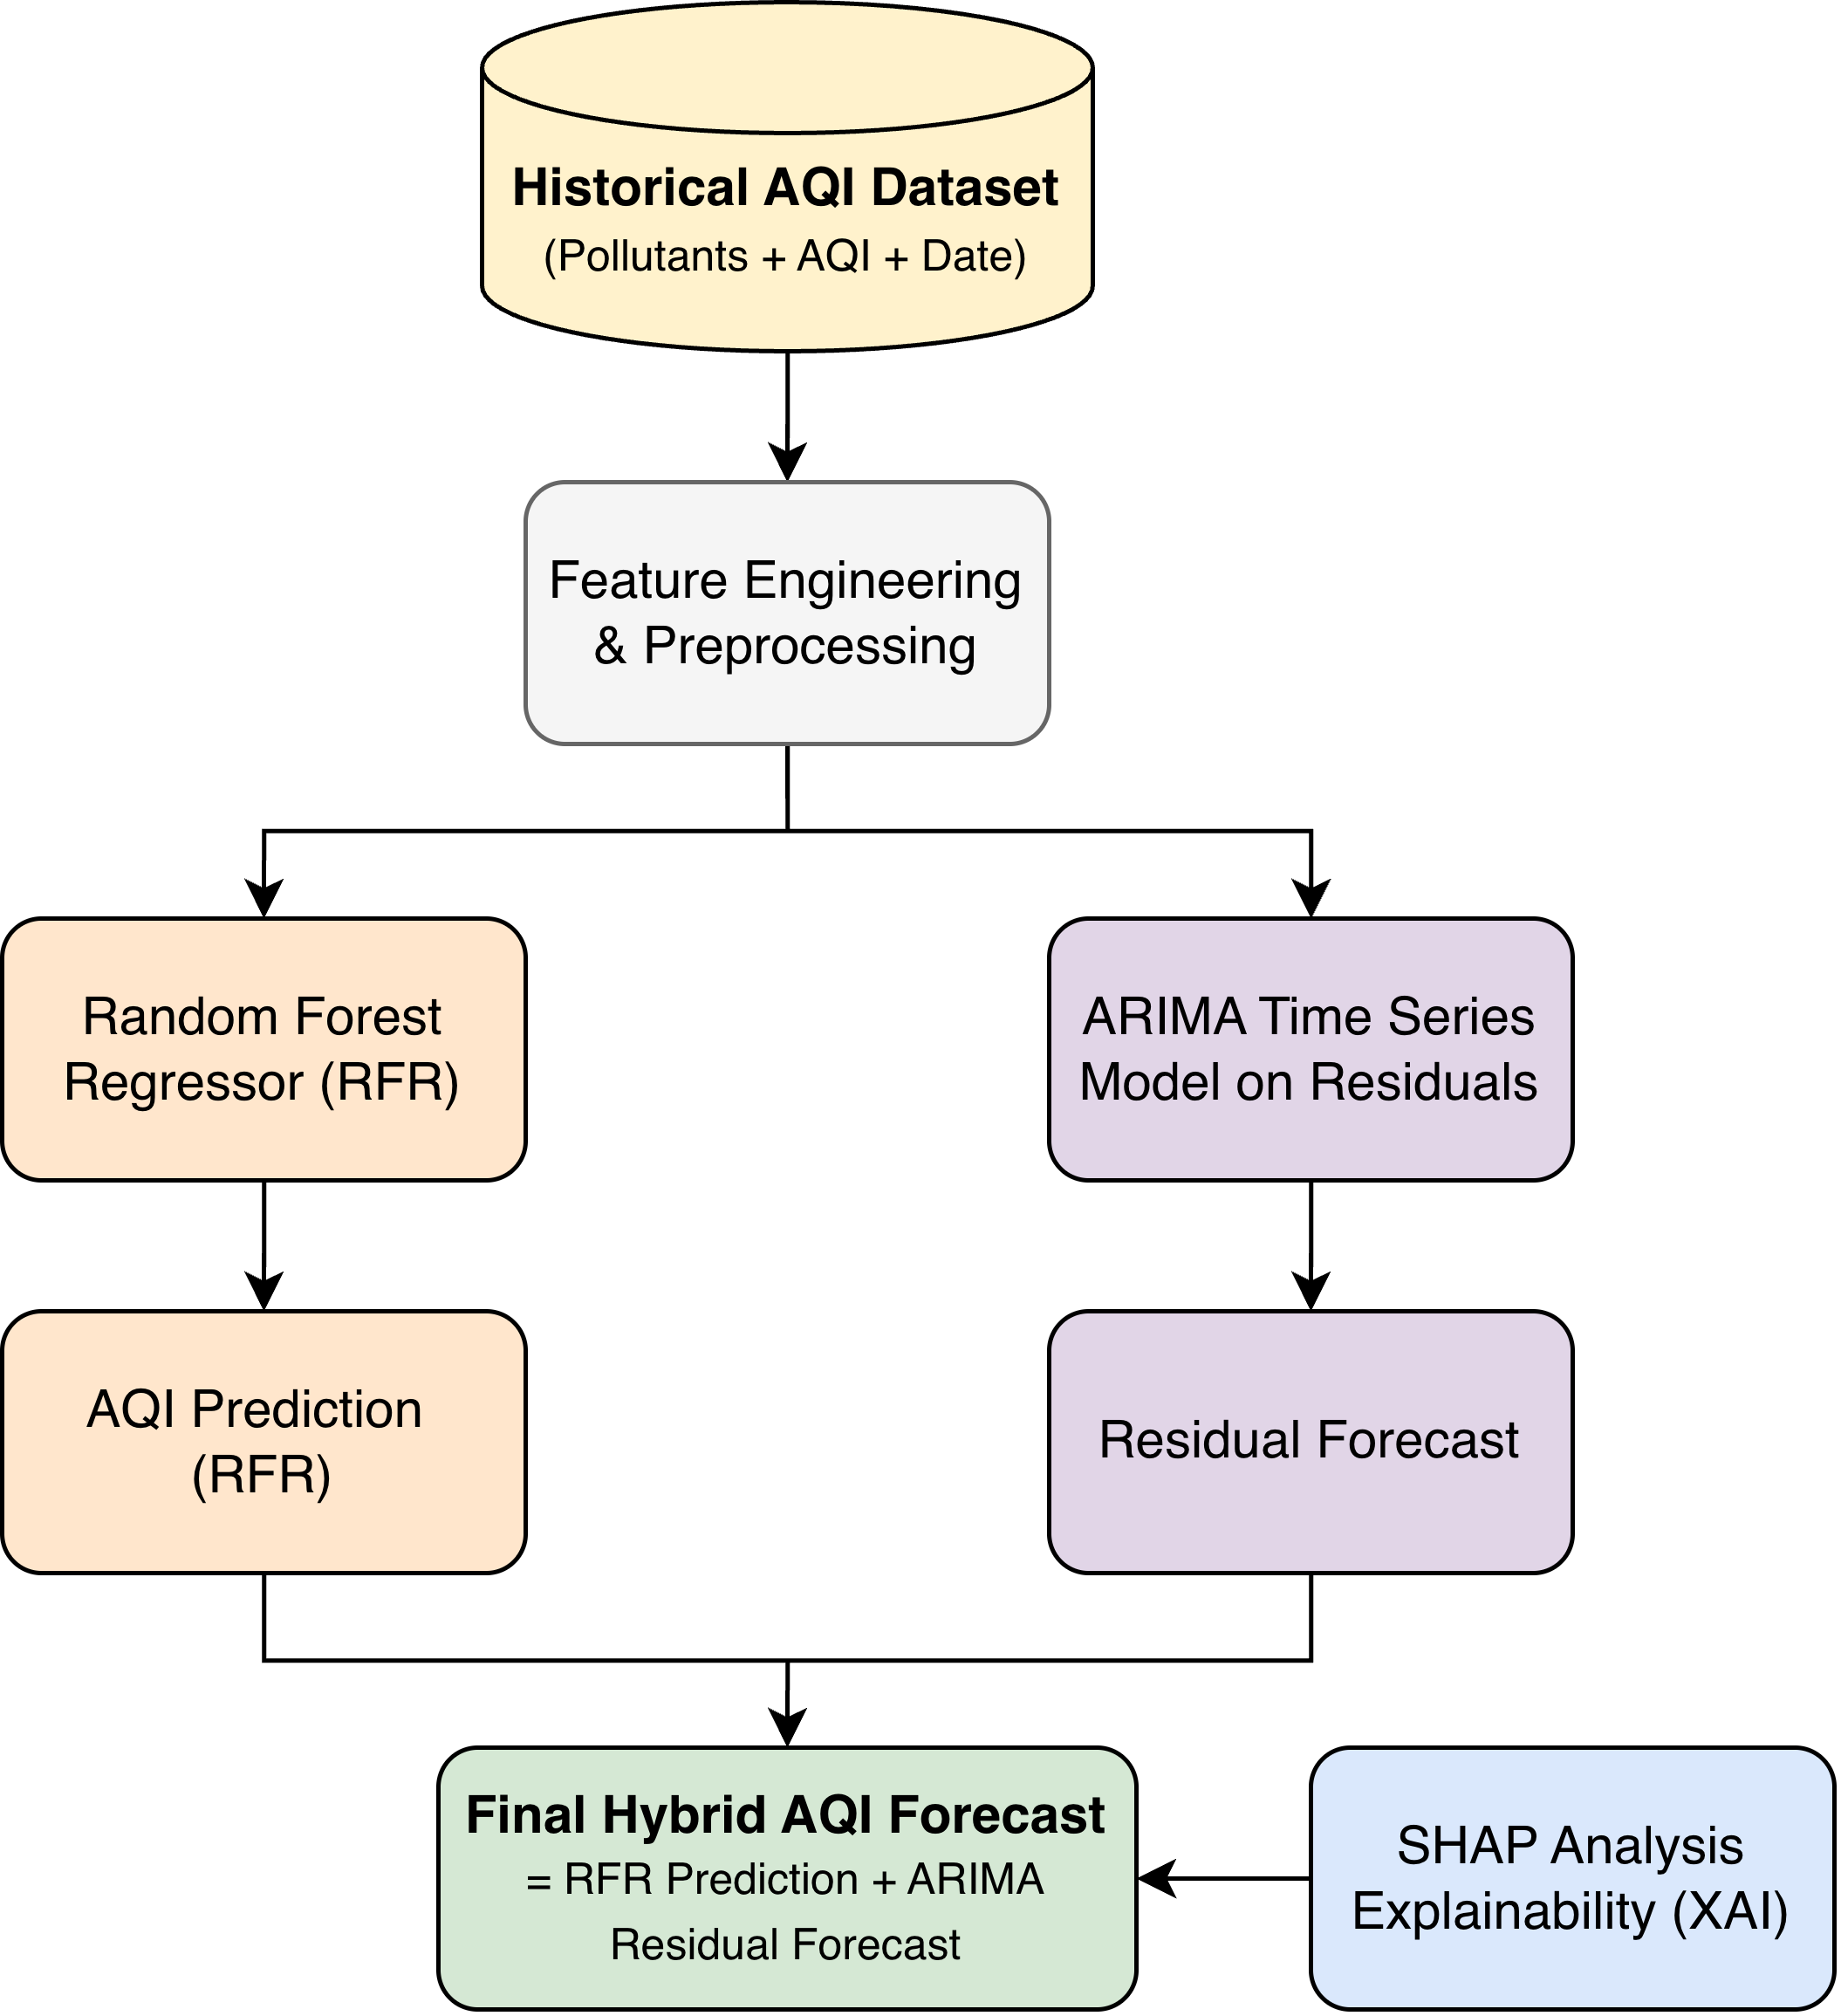
\includegraphics[width=0.5\textwidth]{images/gambar2.png}
  \caption{Arsitektur Aliran Kerja Model Hibrida \textit{Random Forest}-ARIMA \autocite{yenkikar2025explainable}}
  \label{gambar:hybrid}
\end{figure}

\section{Rekayasa Fitur (\textit{Feature Engineering}) Dimensi Atmosferik}

Batasan dari beberapa pemodelan estimasi kualitas udara terdahulu terletak pada penggunaan data historis secara langsung tanpa melalui tahapan rekayasa fitur (\textit{feature engineering}). Konsentrasi polutan di atmosfer dipengaruhi oleh dinamika lingkungan lokal. Penelitian oleh \textcite{naz2024two} menunjukkan bahwa ketidakhadiran tahapan rekayasa fitur dapat memengaruhi nilai galat estimasi karena model mengalami keterbatasan dalam mengidentifikasi hubungan empiris dari variabel prediktor.

Oleh karena itu, rekayasa fitur digunakan untuk mentransformasi data dasar menjadi variabel turunan (\textit{engineered features}) yang merepresentasikan variasi temporal dan karakteristik hubungan polutan. Proses ini mencakup pembentukan fitur jeda temporal (\textit{temporal lags}) untuk memetakan pengaruh variabel dari periode sebelumnya, metrik tren berjalan untuk mengamati volatilitas data, serta fitur interaksi komposit untuk mendeteksi indikasi kondisi atmosferik tertentu. Transformasi ini ditujukan untuk membantu algoritma \textit{machine learning} dalam mengenali karakteristik data secara lebih terstruktur.

\subsection{Kalkulasi Jeda Temporal (\textit{Lag Features})}

Pemodelan deret waktu untuk kualitas udara didasarkan pada asumsi bahwa nilai konsentrasi polutan pada waktu saat ini ($t$) memiliki ketergantungan terhadap nilai pada rentang waktu sebelumnya ($t-k$). Keterikatan temporal ini terjadi karena partikulat (seperti PM\textsubscript{10}) mengalami proses peluruhan secara bertahap di atmosfer. Oleh karena itu, mentransformasi data observasi masa lalu menjadi variabel masukan melalui fitur jeda temporal (\textit{lag features}) digunakan sebagai mekanisme untuk menyertakan informasi dependensi temporal pada algoritma.

Pembentukan fitur jeda jangka pendek, yaitu \textit{lag-1} (satu hari sebelumnya) dan \textit{lag-2} (dua hari sebelumnya), dirancang untuk memetakan pengaruh sisa polutan harian. Fluktuasi nilai PM\textsubscript{10} pada hari ini dipengaruhi oleh akumulasi polutan hari sebelumnya yang tertahan di lapisan atmosfer bawah akibat fenomena inversi suhu. Melalui penambahan variabel ini, algoritma dapat mengidentifikasi kecenderungan akumulasi polutan di suatu wilayah.

Selain itu, fitur jeda jangka menengah seperti \textit{lag-7} (tujuh hari sebelumnya) disertakan untuk mendeteksi siklus aktivitas mingguan. Di wilayah urban seperti Jakarta, aktivitas transportasi dan industri menunjukkan perbedaan karakteristik pola antara hari kerja (\textit{weekdays}) dan akhir pekan (\textit{weekends}). Fitur \textit{lag-7} menggunakan penanda fungsional agar model mengenali siklus periodik mingguan tersebut agar dapat mengantisipasi pola variasi mobilitas masyarakat perkotaan.

\subsection{Metrik Tren Berjalan (\textit{Rolling Window Statistics})}

Data kualitas udara harian dapat mengandung fluktuasi acak (\textit{noise}) akibat faktor meteorologi sesaat. Jika model prediksi hanya menggunakan nilai observasi tunggal seperti fitur jeda (\textit{lag}), model tersebut berpotensi mengalami \textit{overfitting} karena algoritma menjadi sensitif terhadap fluktuasi jangka pendek dan kurang mampu mengidentifikasi kecenderungan pergerakan data secara keseluruhan.

Untuk meminimalkan risiko tersebut, rekayasa fitur diperluas dengan menambahkan perhitungan statistik berbasis rentang waktu berjalan (\textit{rolling window statistics}). Metode ini berfungsi untuk mentransformasi fluktuasi harian menjadi nilai tren pergerakan akumulasi polutan. Fitur ini dihitung melalui dua pendekatan, yaitu rata-rata bergerak (\textit{rolling mean}) dan standar deviasi bergerak (\textit{rolling standard deviation}).

\newpage

Pendekatan rata-rata bergerak (\textit{moving average}) digunakan untuk memperhalus fluktuasi harian yang ekstrim pada data. Fitur ini menyajikan representasi mengenai arah pergerakan tren polutan secara umum. Pada penelitian ini, digunakan jendela waktu berjalan 3-hari (\texttt{pm10\_ma3}) untuk mengidentifikasi tren jangka pendek dan jendela 7-hari (\texttt{pm10\_ma7}) untuk mengevaluasi stabilitas tren mingguan. Formulasi matematika untuk menghitung rata-rata bergerak pada rentang waktu $w$ diturunkan pada Persamaan \ref{eq:ma_feature}.

\begin{equation}
MA_w(t) = \frac{1}{w} \sum_{i=1}^{w} y_{t-i}
\label{eq:ma_feature}
\end{equation}
\eqcaption{Formulasi Kalkulasi \textit{Moving Average} Berbasis Jendela Waktu}

Sementara itu, pendekatan standar deviasi bergerak (\textit{rolling standard deviation}) berfungsi untuk mengukur derajat volatilitas data. Karakteristik stabilitas atmosfer dapat mengalami variasi seiring dengan perubahan cuaca harian. Penambahan variabel \texttt{pm10\_std7} digunakan sebagai indikator bagi model untuk mendeteksi keberadaan fluktuasi yang besar pada data. Perhitungan standar deviasi ini diturunkan pada Persamaan \ref{eq:std_feature}.

\begin{equation}
STD_w(t) = \sqrt{\frac{1}{w-1} \sum_{i=1}^{w} \left( y_{t-i} - MA_w(t) \right)^2}
\label{eq:std_feature}
\end{equation}
\eqcaption{Formulasi Derivasi \textit{Rolling Standard Deviation}}
\subsection{Penanda Temporal Kategorikal dan Interaksi Polutan}

Model juga memerlukan variabel temporal eksplisit untuk mengenali pengaruh pergantian musim. Fitur kategorikal \texttt{month} (bulan) dan \texttt{season} (musim) digunakan agar algoritma dapat mempelajari pola pengendapan basah (\textit{wet scavenging}) di mana curah hujan berkontribusi menurunkan konsentrasi polutan di udara. Selain itu, variabel biner \texttt{is\_weekend} ditambahkan sebagai penanda komputasi mengenai penurunan volume kendaraan pada akhir pekan.

Untuk aspek kimiawi, pembentukan partikulat sangat dipengaruhi oleh reaksi fotokimiawi akibat radiasi sinar matahari. Fitur interaksi komposit \texttt{co\_times\_o3} (hasil perkalian konsentrasi Karbon Monoksida dengan Ozon) dimasukkan sebagai variabel baru. Karbon Monoksida merepresentasikan indikator emisi primer kendaraan, sedangkan Ozon merupakan indikator derajat oksidasi atmosferik. Melalui penggabungan kedua nilai tersebut menjadi fitur tunggal, model \textit{Random Forest} dapat mengidentifikasi kondisi pembentukan polutan sekunder secara lebih efisien tanpa memerlukan kedalaman percabangan pohon keputusan yang tinggi.

\subsection{Spesifikasi Matriks Fitur Prediktor}

Proses rekayasa fitur dalam penelitian ini disusun menjadi sebuah himpunan variabel masukan (\textit{feature matrix}). \textcite{naz2024two} mengonfirmasi bahwa penerapan rekayasa fitur secara tepat dapat memberikan kontribusi positif terhadap performa model prediksi deret waktu kualitas udara.

Matriks fitur pada penelitian ini terdiri dari 15 variabel yang dikelompokkan ke dalam 5 fitur dasar (\textit{baseline}) dan 10 fitur turunan (\textit{engineered features}). Keseluruhan spesifikasi dari kelima belas fitur masukan tersebut beserta fungsi fisisnya disajikan pada Tabel \ref{tbl:features}.

\setlength{\tabcolsep}{5pt} 
\begin{longtable}{>{\raggedright\arraybackslash}p{2.5cm}
                   >{\raggedright\arraybackslash}p{2.3cm}
                   >{\raggedright\arraybackslash}p{8.1cm}}
\caption{Spesifikasi Matriks 15 Fitur Prediktor dalam Arsitektur Model} \label{tbl:features} \\

\toprule
\textbf{Kategori} & \textbf{Nama Fitur} & \textbf{Deskripsi dan Fungsi Fisis Atmosferik} \\
\midrule
\endfirsthead

\multicolumn{3}{c}{\tablename\ \thetable\ Spesifikasi Matriks 15 Fitur Prediktor (Lanjutan)} \\
\toprule
\textbf{Kategori} & \textbf{Nama Fitur} & \textbf{Deskripsi dan Fungsi Fisis Atmosferik} \\
\midrule
\endhead

\midrule
\multicolumn{3}{r}{\textit{Bersambung ke halaman berikutnya.}} \\
\endfoot

\bottomrule
\endlastfoot

\textit{Baseline} & pm10 & Konsentrasi harian PM\textsubscript{10} aktual. \\
\textit{Baseline} & so2 & Konsentrasi Sulfur Dioksida (SO\textsubscript{2}). \\
\textit{Baseline} & co & Konsentrasi Karbon Monoksida (CO) sebagai indikator emisi primer transportasi. \\
\textit{Baseline} & o3 & Konsentrasi Ozon Permukaan (O\textsubscript{3}) sebagai indikator aktivitas fotokimia. \\
\textit{Baseline} & no2 & Konsentrasi Nitrogen Dioksida (NO\textsubscript{2}). \\
\textit{Lag} Temporal & pm10\_lag1 & Nilai PM\textsubscript{10} hari $t-1$ untuk menangkap pengaruh persistensi polutan. \\
\textit{Lag} Temporal & pm10\_lag2 & Nilai PM\textsubscript{10} hari $t-2$. \\
\textit{Lag} Temporal & pm10\_lag7 & Nilai PM\textsubscript{10} hari $t-7$ untuk memetakan pola perulangan mingguan. \\
\textit{Statistik Berjalan} & pm10\_ma3 & Rata-rata bergerak 3 hari untuk mereduksi fluktuasi jangka pendek. \\
\textit{Statistik Berjalan} & pm10\_ma7 & Rata-rata bergerak 7 hari untuk mengevaluasi stabilitas satu minggu. \\
\textit{Statistik Berjalan} & pm10\_std7 & Standar deviasi bergerak 7 hari untuk mengukur tingkat volatilitas data. \\
\textit{Kategorikal} & month & Penanda bulan (1--12) untuk memetakan variasi musiman makro. \\
\textit{Kategorikal} & is\_weekend & Indikator biner akhir pekan (0/1) untuk meninjau perubahan mobilitas urban. \\
\textit{Kategorikal} & season & Klasifikasi musim hujan/kemarau sebagai representasi efek pengendapan basah. \\
\textit{Interaksi Kimia} & co\_times\_o3 & Hasil kali CO $\times$ O\textsubscript{3} untuk mendeteksi laju pembentukan polutan sekunder. \\
\end{longtable}

\section{Prosedur Penyetelan Parameter Menggunakan Optuna}

Dalam pengembangan model pembelajaran mesin, penyesuaian nilai parameter internal (\textit{hyperparameter}) merupakan tahapan pendukung untuk memfasilitasi proses pelatihan komponen pembentuk model hibrida. Pada algoritma \textit{Random Forest}, tahapan ini mencakup pengaturan batasan struktural seperti jumlah pohon keputusan dan batas kedalaman cabang. Penentuan nilai parameter ini diterapkan sebagai instrumen bantu untuk mengendalikan kondisi di mana model meniru data latih secara berlebihan (\textit{overfitting}) atau kurang mampu menangkap pola dasar data (\textit{underfitting}). Pustaka Optuna digunakan dalam penelitian ini sebagai alat pendukung untuk mencari konfigurasi parameter secara terarah berdasarkan riwayat eksperimen sebelumnya, guna membantu proses inisialisasi komponen non-linier pada arsitektur hibrida \autocite{kostadinov2024forecasting}.

\subsection{Perbandingan Metode Grid Search dan Pencarian Probabilistik}

Metode \textit{Grid Search} bekerja dengan mengevaluasi seluruh kombinasi parameter yang ditentukan dalam ruang pencarian secara berurutan. Pendekatan konvensional ini memerlukan alokasi waktu pemrosesan yang bertambah seiring banyaknya variasi parameter yang diuji. Sebagai alternatif pendukung, pencarian berbasis probabilitas memanfaatkan data evaluasi dari tahapan sebelumnya untuk memperkirakan rentang parameter berikutnya yang memiliki potensi nilai kesalahan harian yang lebih rendah. Pustaka Optuna menerapkan prinsip ini dengan membangun fungsi perkiraan (\textit{surrogate model}) untuk memetakan pengaruh nilai parameter terhadap nilai galat estimasi, sehingga durasi pencarian konfigurasi pada komponen model hibrida dapat berjalan secara teratur \autocite{kostadinov2024forecasting}.

\newpage

\subsection{Mekanisme Pencarian Berbasis \textit{Tree-structured Parzen Estimator} (TPE)}

Algoritma \textit{Tree-structured Parzen Estimator} (TPE) di dalam pustaka Optuna memisahkan hasil evaluasi parameter dari tahapan sebelumnya ke dalam dua kelompok distribusi secara statistik, yaitu kelompok dengan nilai galat rendah dan kelompok dengan nilai galat tinggi. Rekomendasi nilai parameter baru kemudian diarahkan secara probabilistik pada area ruang parameter yang mendekati karakteristik kelompok galat rendah. Prosedur ini difungsikan untuk membantu proses kalibrasi parameter pembentuk arsitektur hibrida.

\subsection{Prosedur Pemangkasan Percobaan (\textit{Pruning})}

Pencarian parameter didukung oleh prosedur pemangkasan otomatis (\textit{pruning}). Mekanisme ini mengevaluasi perkembangan nilai galat di pertengahan proses pelatihan suatu urutan percobaan. Jika pada tahapan awal nilai galat yang dihasilkan menunjukkan kecenderungan yang lebih besar dibandingkan riwayat percobaan sebelumnya, proses komputasi untuk kombinasi parameter tersebut akan dihentikan secara dini. Langkah ini digunakan untuk menghemat penggunaan sumber daya memori tanpa memengaruhi hasil akhir pencarian parameter pendukung model.

\section{Skalabilitas dan Kompleksitas Komputasi Algoritma}

Evaluasi terhadap sebuah arsitektur pemodelan \textit{machine learning} tidak hanya diukur berdasarkan akurasi statistik, tetapi juga berdasarkan skalabilitas komputasinya. Analisis kompleksitas komputasi digunakan sebagai standar pengukuran untuk memperkirakan kecenderungan kebutuhan memori (\textit{space complexity}) dan waktu pemrosesan (\textit{time complexity}) seiring dengan bertambahnya volume data masukan.

Estimasi efisiensi algoritma ini diformulasikan menggunakan notasi \textit{Big-O} ($O$). Notasi ini mendeskripsikan batas atas waktu eksekusi (\textit{upper bound}) atau performa algoritma pada skenario terburuk (\textit{worst-case scenario}) ketika ukuran data observasi ($N$) bernilai besar. Melalui pendekatan teoretis ini, potensi kendala efisiensi komputasi dapat diidentifikasi sebelum model diterapkan pada tahap implementasi operasional ke dalam sistem peladen (\textit{server}).

Pada kasus peramalan kualitas udara harian di Jakarta, sistem memerlukan proses kalkulasi yang cepat secara berulang (iteratif) setiap hari. Oleh karena itu, penggabungan model pada arsitektur hibrida \textit{Random Forest}-ARIMA harus dipastikan secara teoritis tidak menghasilkan pertumbuhan durasi eksekusi yang eksponensial.

\newpage

\subsection{Kompleksitas Komputasi Fase Primer: \textit{Random Forest}}

Kompleksitas waktu untuk proses pelatihan (\textit{training time}) pada algoritma \textit{Random Forest} ditentukan oleh interaksi tiga variabel utama, yaitu total jumlah baris data observasi ($N$), jumlah fitur prediktor yang dievaluasi pada setiap penentuan cabang ($M$), dan jumlah pohon keputusan yang dibangun dalam model (\textit{estimators}) yang disimbolkan dengan $K$. Ketiga parameter ini menentukan jumlah operasi perhitungan yang dieksekusi oleh prosesor komputer.

Dalam proses pembangunan satu pohon keputusan, tahapan dengan kebutuhan komputasi terbesar adalah proses pengurutan (\textit{sorting}) nilai fitur untuk menemukan titik pisah (\textit{threshold}) dengan nilai kesalahan minimum. Algoritma \textit{sorting} secara umum memerlukan waktu komputasi sebesar $N \log N$. Proses ini kemudian dikalikan dengan jumlah fitur ($M$) dan jumlah pohon yang dibangun ($K$). Dengan demikian, kompleksitas waktu batas atas untuk pelatihan \textit{Random Forest} diturunkan pada Persamaan \ref{eq:complexity_rf}.

\begin{equation}
    O(K \cdot M \cdot N \log N)
\label{eq:complexity_rf}
\end{equation}
\eqcaption{Formulasi Kompleksitas Waktu Pelatihan \textit{Random Forest}}

Berdasarkan Persamaan \ref{eq:complexity_rf}, \textit{Random Forest} memiliki kompleksitas waktu bersifat kuasi-linier ($N \log N$). Waktu komputasinya mengalami pertumbuhan yang konstan seiring dengan penambahan baris data. Karakteristik skalabilitas ini mendukung efisiensi \textit{Random Forest} untuk memproses data tabular berjumlah besar jika dibandingkan dengan arsitektur \textit{Deep Learning} seperti LSTM yang memiliki kompleksitas fungsi kuadratik $O(N^2)$ serta memerlukan proses perulangan mundur (\textit{backpropagation}) secara berulang.

\subsection{Kompleksitas Komputasi Fase Sekunder: Arsitektur ARIMA}

Pada fase sekunder, pemrosesan sisa galat dilakukan menggunakan algoritma statistik ARIMA. Karakteristik komputasi ARIMA berbeda dengan arsitektur pohon keputusan. ARIMA tidak melakukan pemisahan variabel fitur, melainkan berfokus pada penyelesaian fungsi estimasi matematis berupa \textit{Maximum Likelihood Estimation} (MLE). Fungsi MLE bertujuan menemukan kombinasi koefisien pembobotan yang mendekati pola data sisaan (\textit{residuals}) aktual.

Kompleksitas konvergensi dari fungsi MLE dipengaruhi oleh penjumlahan orde \textit{AutoRegressive} ($p$) dan orde \textit{Moving Average} ($q$), serta total baris deret waktu observasi ($N$). Jika proses perulangan internal pencarian dibatasi oleh konstanta maksimal sebesar $c$, maka batas atas kompleksitas waktu pelatihan algoritma ARIMA direpresentasikan pada Persamaan \ref{eq:complexity_arima}.

\begin{equation}
    O(c \cdot N \cdot (p+q)^2)
\label{eq:complexity_arima}
\end{equation}
\eqcaption{Formulasi Batas Atas Kompleksitas Pelatihan Algoritma ARIMA}

Persamaan \ref{eq:complexity_arima} menunjukkan karakteristik matematis di mana waktu proses ARIMA tumbuh secara linier $O(N)$ terhadap panjang riwayat data. Pertumbuhan waktu berbentuk fungsi kuadratik terjadi pada elemen orde model $(p+q)^2$. Namun, dalam penerapan praktis pemodelan deret waktu, total penjumlahan orde $p$ dan $q$ umumnya bernilai kecil. Dengan karakteristik tersebut, penambahan tahap ARIMA di akhir rangkaian sistem estimasi memiliki kebutuhan komputasi yang rendah dan tidak menghambat siklus pembaruan kalkulasi harian.

\section{Interpretabilitas Model menggunakan SHAP}

Meskipun model ansambel seperti \textit{Random Forest} memberikan nilai akurasi estimasi yang terkendali, model ini memiliki karakteristik komputasi yang tertutup (\textit{black-box}) \autocite{jimenez2024explainable}. Untuk kebutuhan analisis polusi udara, model harus mampu memberikan penjelasan mengenai variabel fitur yang memengaruhi variasi nilai konsentrasi PM\textsubscript{10}. Penelitian ini menerapkan pendekatan \textit{Explainable AI} (XAI) melalui metode SHAP (\textit{SHapley Additive exPlanations}) untuk memetakan besaran pengaruh setiap variabel masukan terhadap hasil estimasi akhir.

\subsection{Justifikasi Validitas SHAP pada Model Hibrida Sekuensial}
Satu hal krusial yang perlu diklarifikasi adalah mengapa metode SHAP valid digunakan untuk menginterpretasikan model hibrida sekuensial ini. 

Dalam arsitektur hibrida yang diusulkan, seluruh 15 variabel masukan (fitur dasar, lag temporal, statistik jendela berjalan, penanda musim, dan interaksi komposit $CO \times O_3$) dievaluasi dan diproses hanya pada fase primer oleh model regresi non-linier Random Forest. Model ARIMA pada fase sekunder tidak menerima 15 fitur tersebut, melainkan hanya menerima data univariate deret waktu sisaan (residual) satu dimensi ($e_t$) yang tidak memiliki struktur fitur regresi. 

Oleh karena itu, hubungan inferensial pemetaan fitur-fitur prediktor terhadap keputusan estimasi sepenuhnya terjadi di dalam struktur pohon keputusan \textit{Random Forest}. Penerapan TreeSHAP secara eksklusif pada fase primer bersifat valid karena mengurai visualisasi kontribusi marginal dari 15 fitur tersebut terhadap pembentukan nilai prediksi awal ($\hat{N}_t$), yang merupakan komponen varians terbesar dalam arsitektur hibrida ini. Koreksi residual dari ARIMA bersifat post-hoc penyesuaian tren runtun waktu linear sisa dan tidak mengaburkan interpretasi fisis antar-fitur polutan yang diekstrak oleh SHAP.

\subsection{Distribusi Atribusi \textit{Shapley Value}}

Mekanisme perhitungan distribusi bobot ini didasarkan pada perhitungan nilai Shapley (\textit{Shapley Value}). Algoritma terlebih dahulu menghitung efek marjinal (\textit{marginal effect}), yaitu seberapa besar hasil prediksi berubah ketika sebuah fitur tertentu ($i$) dimasukkan ke dalam sebuah himpunan fitur ($S$) yang tidak mengandung fitur $i$. Perhitungan efek marjinal ini direpresentasikan pada Persamaan \ref{eq:shap_marginal}.

\begin{equation}
\Delta f_i(S) = f(S \cup \{i\}) - f(S)
\label{eq:shap_marginal}
\end{equation}
\eqcaption{Formulasi Diferensiasi Kontribusi Marjinal Fitur Tunggal}

Nilai akhir bobot atribusi SHAP ($\phi_i$) diperoleh dengan menghitung rata-rata terbobot dari semua kemungkinan efek marjinal tersebut melalui probabilitas permutasi untuk meminimalkan bias urutan variabel masukan, sebagaimana diturunkan pada Persamaan \ref{eq:shap_math}.

\begin{equation}
\phi_i = \sum_{S \subseteq N \setminus \{i\}} \frac{|S|!(|N|-|S|-1)!}{|N|!} \left[ f(S \cup \{i\}) - f(S) \right]
\label{eq:shap_math}
\end{equation}
\eqcaption{Formulasi Agregasi \textit{Shapley Value}}

\subsection{Interpretasi Visual Diagnostik SHAP}

Keluaran dari perhitungan nilai SHAP dapat ditampilkan melalui dua grafik utama untuk membantu proses interpretasi model, yaitu \textit{SHAP Summary Plot} (\textit{Beeswarm}) dan \textit{SHAP Dependence Plot}.

\textit{SHAP Summary Plot} (\textit{Beeswarm}) digunakan untuk menampilkan peringkat dan arah pengaruh dari setiap variabel masukan terhadap prediksi model secara global. Pada grafik ini, sumbu vertikal ($Y$) menampilkan nama fitur yang diurutkan berdasarkan kontribusi absolutnya terhadap model. Sumbu horizontal ($X$) menunjukkan besaran nilai SHAP yang dihasilkan. Grafik ini menggunakan gradasi warna untuk menunjukkan nilai asli dari fitur tersebut, di mana warna biru merepresentasikan nilai fitur yang rendah dan warna merah merepresentasikan nilai fitur yang tinggi. Sebagai contoh, jika persebaran titik berwarna merah pada fitur Ozon berada di sisi kanan sumbu $X$ (nilai SHAP positif), kondisi tersebut menunjukkan bahwa nilai konsentrasi Ozon yang tinggi berhubungan dengan estimasi nilai \MakeUppercase{pm}\textsubscript{10} yang lebih tinggi pada model.

Sementara itu, \textit{SHAP Dependence Plot} digunakan untuk menganalisis efek dari satu variabel fitur secara spesifik. Sumbu horizontal memuat nilai asli fitur tersebut, sedangkan sumbu vertikal memuat nilai dampak SHAP terhadap prediksi model. Distribusi titik pada grafik memperlihatkan karakteristik hubungan fitur terhadap target, seperti kecenderungan pola linear, eksponensial, atau kondisi konstan pada titik tertentu. \textit{SHAP Dependence Plot} juga dapat dilengkapi dengan gradasi warna berbasis variabel kedua untuk meninjau pola interaksi antara dua variabel prediktor dalam memengaruhi hasil estimasi.

\section{Prosedur Pengukuran Galat dan Skema Validasi Temporal}

Pengukuran nilai galat peramalan kualitas udara merupakan tahapan kontrol untuk menguji keandalan hasil estimasi model hibrida. Mengingat data konsentrasi PM\textsubscript{10} memiliki karakteristik fluktuasi yang dipengaruhi faktor harian, diperlukan metrik evaluasi statistik untuk mengamati deviasi hasil prediksi terhadap data aktual. Penelitian ini menggunakan tiga indikator ukuran standar, yaitu \textit{Root Mean Square Error} (RMSE), \textit{Mean Absolute Error} (MAE), dan Koefisien Determinasi ($R^2$), yang digabungkan dengan skema validasi berbasis waktu untuk menjaga proses evaluasi agar terhindar dari kebocoran data masa depan (\textit{look-ahead bias}).

\subsection{Metrik \textit{Root Mean Square Error} (RMSE)}

Metrik \textit{Root Mean Square Error} (RMSE) menghitung akar kuadrat dari rata-rata selisih kuadrat antara nilai hasil estimasi model dengan nilai observasi aktual. Karena melibatkan operasi pengkuadratan selisih, RMSE memberikan bobot penalti yang lebih besar pada nilai kesalahan yang besar (\textit{outliers}). Karakteristik ini digunakan sebagai indikator kontrol untuk mengamati ketahanan model hibrida saat menghadapi fluktuasi data yang tajam pada set pengujian.

\subsection{Metrik \textit{Mean Absolute Error} (MAE) dan Koefisien Determinasi ($R^2$)}

Sebagai pelengkap analisis, metrik \textit{Mean Absolute Error} (MAE) digunakan untuk mengukur rata-rata mutlak dari kesalahan estimasi secara linier proporsional. Metrik ini menggambarkan deviasi rata-rata harian hasil prediksi terhadap kondisi riil di lapangan. Sementara itu, Koefisien Determinasi ($R^2$) digunakan untuk mengamati seberapa besar variabilitas data target dapat digambarkan oleh variabel masukan di dalam model, dengan rentang nilai antara 0 hingga 1.

\subsection{Skema Validasi Temporal \textit{Time-Series Forward Chaining}}

Prosedur pembagian data latih dan data uji pada data deret waktu memerlukan penanganan khusus untuk menjaga urutan kronologis data. Penggunaan metode validasi silang konvensional (\textit{K-Fold Cross-Validation}) yang mengacak baris data kurang sesuai karena dapat menimbulkan risiko kebocoran data masa depan (\textit{look-ahead bias}), di mana model secara tidak langsung mempelajari informasi periode mendatang untuk memprediksi periode masa lalu. Guna menjaga validitas pengujian model hibrida, digunakan skema \textit{TimeSeriesSplit} dengan pendekatan rantaian maju (\textit{Forward Chaining}). Dalam prosedur ini, data pembagi bergerak maju secara kronologis berurutan, sehingga model selalu diuji menggunakan data periode setelah masa pelatihan, menyimulasikan kondisi operasional rill saat menerima data baru harian.